\documentclass[10pt]{article} % For LaTeX2e
\usepackage{tmlr}
% If accepted, instead use the following line for the camera-ready submission:
%\usepackage[accepted]{tmlr}
% To de-anonymize and remove mentions to TMLR (for example for posting to preprint servers), instead use the following:
%\usepackage[preprint]{tmlr}

% Optional math commands from https://github.com/goodfeli/dlbook_notation.
\input{math_commands.tex}

\usepackage{hyperref}
\usepackage{url}
\usepackage{graphicx}
\usepackage{booktabs}
\usepackage{amsmath}

\title{Revisiting Bilinear MLP Interpretability: \\A Reproduction and Extension Study}

% Authors must not appear in the submitted version. They should be hidden
% as long as the tmlr package is used without the [accepted] or [preprint] options.
% Non-anonymous submissions will be rejected without review.

\author{\name Ippokratis Pantelidis \email ippokratis.pantelidis@student.uva.nl \\
      \addr University of Amsterdam}

\def\month{MM}  % Insert correct month for camera-ready version
\def\year{YYYY} % Insert correct year for camera-ready version
\def\openreview{\url{https://openreview.net/forum?id=XXXX}} % Insert correct link to OpenReview for camera-ready version

\begin{document}

\maketitle

\begin{abstract}
Bilinear multilayer perceptrons (MLPs) replace element-wise nonlinearities with the
element-wise product of two linear maps, which makes the layer's computation an exact
quadratic form in its input. \citet{pearce2025bilinear} showed that eigendecomposing
the resulting interaction matrices, using the weights alone, recovers interpretable
features in image classifiers and traceable circuits in language models. We reproduce
this work across both domains. We organize the paper's contributions into seven
independently testable claims covering feature interpretability, low-rank structure,
the effect of regularization, causal validity of weight-derived features, circuit
discovery, low-rank approximation of sparse autoencoder features, and the practicality
of bilinear layers as a drop-in replacement. Six of the seven claims reproduce; the
seventh reproduces with caveats that we trace to a specific obstacle: the cleaned
TinyStories dataset used to train the published checkpoints was never released, which
distorts absolute loss-based metrics while leaving relative and structural results
intact. We document this and other deviations, including a fine-tuning learning rate
that must differ from the reported pretraining value to avoid divergence. Beyond
reproduction, we extend the framework to variational autoencoders; this part of the
study is described in Section~\ref{sec:extension}. Code, per-experiment results, and
trained artifacts are available in our public repository.
\end{abstract}

\section{Introduction}

Most interpretability methods explain a network through its activations on data.
Saliency maps attribute a single prediction to input pixels \citep{simonyan2014deep},
and sparse dictionary learning decomposes hidden activations over a dataset into more
interpretable atoms \citep{bricken2023monosemanticity, cunningham2024sparse}. Both
families describe what a model does on the inputs we happen to feed it. They say
little about the function stored in the weights, and their conclusions may not hold
off-distribution.

\citet{pearce2025bilinear} take the opposite route. Building on a technical note by
\citet{sharkey2023technical}, they study bilinear MLPs, a variant of the Gated Linear
Unit \citep{shazeer2020glu} without the gate nonlinearity,
\begin{equation}
  g(\vx) = (\mW\vx) \odot (\mV\vx),
\end{equation}
where $\odot$ is the element-wise product. Because no nonlinearity intervenes, the
activation of any output direction is an exact quadratic form $\vx^\top \mQ \vx$ whose
interaction matrix $\mQ$ is built from the weights alone. Eigendecomposing $\mQ$ then
yields orthogonal input directions with real-valued importances, computable without a
single forward pass. The paper demonstrates this on MNIST and Fashion-MNIST
classifiers, and extends it to transformers with bilinear MLP blocks, where
interaction matrices connect sparse autoencoder (SAE) features across a layer and
expose a sentiment-negation circuit directly in the weights.

This paper reports an independent reproduction of that work. We reproduce the main
figures and appendices of \citet{pearce2025bilinear} in both the vision and the
language settings, quantify results that the original presents qualitatively, and
record every deviation we encountered together with its cause. Reproducing the
language experiments required more than rerunning released code: the research
repository behind the paper is no longer public, the cleaned training dataset was
never released, and the vendored library predates breaking changes in its
dependencies. Part of our contribution is documenting how far the published artifacts
alone support the paper's claims, and where the missing pieces matter.

We also extend the framework beyond classification, to variational autoencoders;
Section~\ref{sec:extension} presents this extension.

\section{Scope of reproducibility}
\label{sec:scope}

We organize the contributions of \citet{pearce2025bilinear} into seven claims. Each is
a single testable statement about a different property of bilinear MLPs, so the claims
can be verified or falsified independently. We use the labels C1--C7 throughout the
paper to link experiments to the claims they evaluate.

\begin{itemize}
\item \textbf{C1 --- Interpretability.} Eigendecomposing a trained bilinear MLP's
interaction matrices, using the weights alone and no input data, yields top
eigenvectors that correspond to human-recognizable visual structure, such as digit
strokes on MNIST and garment edges on Fashion-MNIST.

\item \textbf{C2 --- Low rank.} Each class's interaction matrix is effectively
low-rank: truncating the model to its few largest-magnitude eigenvectors preserves
classification accuracy, consistently across model sizes, and the retained
eigenvectors are consistent across training runs.

\item \textbf{C3 --- Regularization shapes features.} The character of the learned
eigenfeatures is controlled by regularization: Gaussian input noise sparsifies and
cleans them, revealing overfitting artifacts in unregularized models, while weight
decay lowers the effective rank; geometric augmentations reshape features in
predictable ways.

\item \textbf{C4 --- Causality.} Eigenvectors are causally meaningful rather than
merely descriptive: adversarial masks constructed purely from the weights, with no
gradients or per-input optimization, reduce accuracy and induce targeted
misclassification far more than matched random masks.

\item \textbf{C5 --- Circuits.} In a bilinear transformer, the interactions that
construct an SAE output feature from SAE input features can be read off the bilinear
tensor directly, recovering an interpretable circuit (the sentiment-negation circuit)
grounded in the weights rather than in gradient-based approximations.

\item \textbf{C6 --- Low-rank approximation of language features.} SAE output features
of bilinear transformers are well approximated by the top one or two eigenvectors of
their interaction matrices, increasingly so the longer the SAE is trained, extending
the low-rank finding of C2 from classifiers to language models.

\item \textbf{C7 --- Practicality.} Adopting bilinear MLPs costs little: they match
gated activations (ReGLU, SwiGLU) in compute-matched language model training, and an
existing SwiGLU transformer can be converted into a bilinear one by fine-tuning the
gate away at a modest loss penalty.
\end{itemize}

Claims C1--C4 concern image classifiers and correspond to Figures~2--7 and
Appendices~A--F and~M of the original paper. Claims C5--C7 concern language models and
correspond to Figures~8--9 and Appendices~G--J and~N--O.

\section{Methodology}
\label{sec:method}

\subsection{Model descriptions}
\label{sec:models}

\paragraph{Bilinear layers and interaction matrices.}
For an input $\vx \in \R^d$, a bilinear layer computes
$g(\vx) = (\mW\vx) \odot (\mV\vx)$ with $\mW, \mV \in \R^{k \times d}$. A single
output $a$ of the layer is $g(\vx)_a = (\vw_{a}^\top \vx)(\vv_{a}^\top \vx) =
\vx^\top (\vw_a \vv_a^\top) \vx$, so the collection of outputs is described by a
third-order tensor with entries $b_{aij} = w_{ai} v_{aj}$. For any output direction
$\vu$, contracting the tensor along the output axis gives an interaction matrix
$\mQ = \vu \cdot_{\text{out}} \tB$, and since only the symmetric part of $\mQ$
contributes to $\vx^\top \mQ \vx$, we symmetrize
$\mQ \leftarrow \tfrac{1}{2}(\mQ + \mQ^\top)$. The spectral theorem then gives
\begin{equation}
  \vx^\top \mQ \vx = \sum_{i=1}^{k} \lambda_i \, (\vv_i^\top \vx)^2,
  \label{eq:eig}
\end{equation}
with orthonormal eigenvectors $\vv_i$ and real eigenvalues $\lambda_i$: the layer's
output along $\vu$ is a weighted sum of squared projections onto orthogonal input
directions. All analyses in this paper are instances of Equation~\ref{eq:eig} for
different choices of $\vu$.

\paragraph{Image classifiers.}
Following the original architecture, the vision models consist of a linear embedding
from $784$ pixels to $d_{\text{hidden}}$ dimensions, a single bilinear layer, and a
linear classification head, with no biases. Unless stated otherwise we use
$d_{\text{hidden}} = 512$; the model-size experiments (C2) sweep
$d_{\text{hidden}} \in \{30, 50, 100, 300, 500, 1000\}$. Eigenvectors are computed in
the embedding space and projected back to pixel space through the embedding weights
for visualization.

\paragraph{Language models.}
The language experiments use the transformer checkpoints released by the original
authors: a 6-layer TinyStories model ($d_{\text{model}} = 512$, $d_{\text{hidden}} =
2048$, 8 heads, context 256, called \emph{ts-tiny} in the paper), and two FineWeb
models following GPT-2 small and medium shapes with 12 and 16 layers
(\emph{fw-small}, \emph{fw-medium}). In all of them the MLP block is bilinear, so the
interaction matrix for any output direction of a block is computable from the
down-projection and the two up-projections. SAE dictionaries with a TopK activation
\citep{gao2024scaling} trained by the original authors on MLP inputs, MLP outputs and
the mid-layer residual stream are likewise public, and we use them unchanged. For C7
we train 6-layer TinyStories transformers from scratch, identical except for the MLP
activation (bilinear, ReGLU, or SwiGLU), and fine-tune the pretrained
TinyLlama-1.1B \citep{zhang2024tinyllama}, whose SwiGLU activation
$x \cdot \sigma(\beta x)$ we anneal from $\beta = 1$ to $\beta = 0$, turning the
gated MLP into a bilinear one.

\subsection{Datasets}
\label{sec:datasets}

\paragraph{MNIST and Fashion-MNIST.} Both datasets contain 70{,}000 grayscale
$28 \times 28$ images in 10 classes with the standard 60{,}000/10{,}000 split
\citep{lecun1998mnist, xiao2017fashion}. Images are normalized to $[0, 1]$ and
flattened.

\paragraph{TinyStories.} The 6-layer transformer and its SAEs were trained by the
original authors on a cleaned, deduplicated version of TinyStories
\citep{eldan2023tinystories} with a custom lowercase 4096-token BPE tokenizer.
The cleaned dataset was never published. We therefore run all
TinyStories evaluations, and our own C7 training runs, on the public
\texttt{roneneldan/TinyStories} corpus, lowercased and tokenized with the authors'
released tokenizer. Section~\ref{sec:deviations} quantifies the consequences.

\paragraph{FineWeb.} For the FineWeb models we sample sequences from the public
\texttt{sample-10BT} configuration of FineWeb \citep{penedo2024fineweb}, tokenized to
length 512 with the Mixtral tokenizer, matching the models' training setup.

\subsection{Hyperparameters}
\label{sec:hyper}

All vision experiments use the training configuration reported in the original paper:
AdamW with learning rate $10^{-3}$, weight decay $1.0$, batch size 2048, cosine
annealing, 50--100 epochs, and additive Gaussian input noise with standard deviation
0.5 unless the experiment sweeps it. The C7 TinyStories runs use the original Table~2
setup (batch 512, context 256, learning rate $10^{-3}$, weight decay 0.1, linear
decay, 5 epochs). Two deliberate deviations, both forced and both documented in
Section~\ref{sec:deviations}, are the fine-tuning learning rate for TinyLlama and the
evaluation dataset for TinyStories models. A complete listing of hyperparameters is
given in Appendix~\ref{app:hyper}.

\subsection{Experimental setup and code}
\label{sec:setup}

Our experiments build on the authors' released library
(\url{https://github.com/tdooms/bilinear-decomposition}), which we vendor unmodified;
every experiment is a self-contained script in our repository that imports from it.
The auxiliary research repository referenced by the paper is no longer available on
GitHub, so all training, evaluation and figure code beyond the library was
re-implemented from the descriptions in the paper. Each experiment writes its figures
alongside a JSON file with its quantitative results, and expensive steps (model
training sweeps, eigendecompositions of up to 8192 SAE features) are cached to disk.

\textbf{C1} trains classifiers on MNIST and Fashion-MNIST and visualizes top
eigenvectors per class (Figures~2--3 of the original; our Figure~\ref{fig:c1}).
\textbf{C2} sweeps six hidden sizes over five seeds each, measures cross-seed cosine
similarity of eigenvectors by rank, and evaluates classifiers truncated to their
top-$k$ eigenvectors per class via Equation~\ref{eq:eig} (original Figure~5 and
Appendix~F). \textbf{C3} sweeps Gaussian input noise, weight decay, and geometric
augmentations, and inspects the resulting eigenvectors and their $(L_1/L_2)^2$
near-sparsity (original Figure~4 and Appendices~B,~E). \textbf{C4} builds adversarial
masks from rows of the pseudoinverse of the top-10 eigenvectors per class, adds them
to test images, and measures accuracy and targeted misclassification against matched
random masks (original Figure~7 and Appendix~M). \textbf{C5} contracts the bilinear
tensor of layer~4 of the TinyStories model with the encoder direction of the
``not-good'' SAE feature, transforms the interaction matrix into the input SAE basis,
and reproduces the interaction submatrix, the eigenvector projection geometry, and
the rank-2 activation approximation (original Figure~8 and Appendices~N,~O).
\textbf{C6} approximates SAE feature activations with truncated eigendecompositions
across the three transformers and across SAEs trained for increasing durations
(original Figure~9, Table~5, Appendix~G). \textbf{C7} trains the three
activation-function variants under identical conditions and logs wall-clock
timestamps with periodic validation, so that both the constant-epochs and the
constant-time comparison of the original Table~6 come from one set of runs, and
fine-tunes TinyLlama with linear $\beta$-annealing over the first 30\% of 100{,}000
steps of roughly 400M FineWeb tokens (original Appendix~J).

Auxiliary analyses of the original paper that are not required to evaluate the seven
claims (per-example explanations, the HOSVD analysis, the reverse-engineering
challenge of the original Figure~6, and the feature-example tables) are also
reproduced and available in the repository.

\subsection{Computational requirements}
\label{sec:compute}

All experiments ran on a shared university server with NVIDIA RTX A5500 GPUs (24~GB).
The vision experiments are light: the largest, the 30-model sweeps behind C2,
complete in about one GPU hour each. The language experiments dominate: regenerating
the eigendecompositions and activations for C6 takes roughly 4 GPU hours, the three
C7 TinyStories runs about 5.3 GPU hours each, and the two TinyLlama fine-tuning arms
about 8 GPU hours each. The full reproduction amounts to approximately 50 GPU hours,
corresponding to an estimated 3.5~kgCO$_2$eq \citep{lacoste2019quantifying}.

\section{Results}
\label{sec:results}

Table~\ref{tab:verdicts} summarizes the outcome per claim; the subsections below give
the evidence. Overall, C1--C5 reproduce, C6 reproduces with one repaired protocol
detail on our side, and C7's within-experiment comparisons reproduce while its
absolute numbers cannot be compared to the original for reasons external to the
method (Section~\ref{sec:deviations}).

\begin{table}[t]
\caption{Summary of reproducibility outcomes per claim.}
\label{tab:verdicts}
\begin{center}
\begin{tabular}{llll}
\toprule
Claim & Setting & Original evidence & Outcome \\
\midrule
C1 interpretability & vision & Figs.~2--3, App.~A & reproduced \\
C2 low rank & vision & Fig.~5, App.~D, F & reproduced \\
C3 regularization & vision & Fig.~4, App.~B, E & reproduced \\
C4 causality & vision & Fig.~7, App.~M & reproduced \\
C5 circuits & language & Fig.~8, App.~N, O & reproduced \\
C6 low-rank approximation & language & Fig.~9, Tab.~5, App.~G, H & reproduced$^{*}$ \\
C7 practicality & language & Tab.~6, Fig.~25, App.~I, J & partially reproduced$^{\dagger}$ \\
\bottomrule
\end{tabular}
\end{center}
\vspace{2pt}
{\small $^{*}$absolute loss-added values (App.~G) are distorted by the unavailable
training dataset; all structural results reproduce.
$^{\dagger}$the small performance gap between activations reproduces; absolute losses
are not comparable, the constant-time equalization did not manifest in our
implementation, and fine-tuning requires a different learning rate than reported
(Section~\ref{sec:deviations}).}
\end{table}

\subsection{C1: top eigenvectors are recognizable visual features}

We train one classifier per dataset with the original configuration and decompose
each class's interaction matrix. Figure~\ref{fig:c1} shows the top positive
eigenvector for classes 1--5 of MNIST and Fashion-MNIST alongside the eigenvalue
spectrum and top eigenvectors for digit~5. The reproduced eigenfeatures match the
original paper's closely: MNIST eigenvectors capture stroke segments specific to each
digit, while Fashion-MNIST eigenvectors act as localized edge detectors, for example
the leg gap of trousers. Because the activation of an eigenvector is quadratic,
$\lambda (\vv^\top \vx)^2$, its sign is arbitrary, and the red and blue regions
implement the XOR-like behavior described in the original: overlap with either region
alone activates the feature, overlap with both cancels. Per-digit spectra for all ten
MNIST classes are reproduced in the repository and match the original Appendix~A.

\begin{figure}[t]
\begin{center}
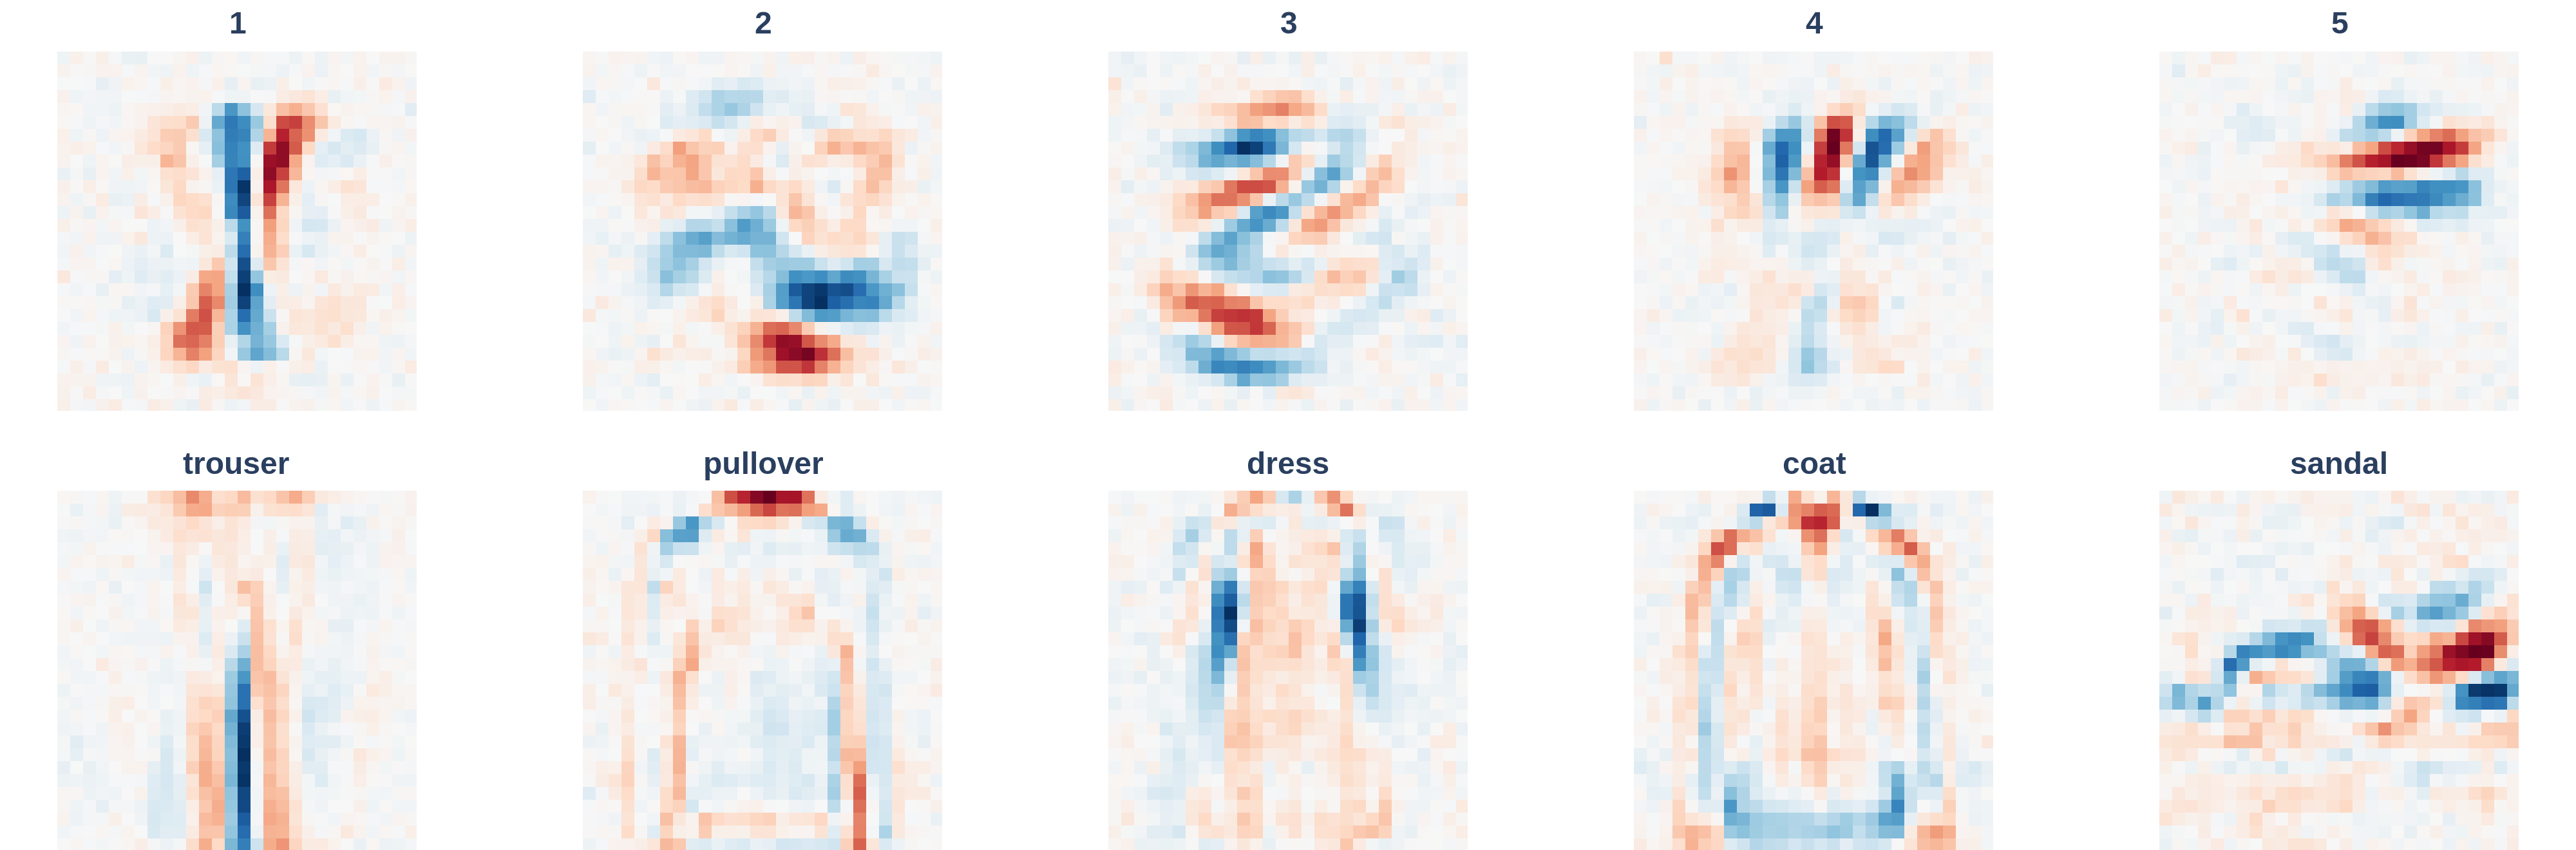
\includegraphics[width=0.95\linewidth]{figures/fig_02.png}\\[4pt]
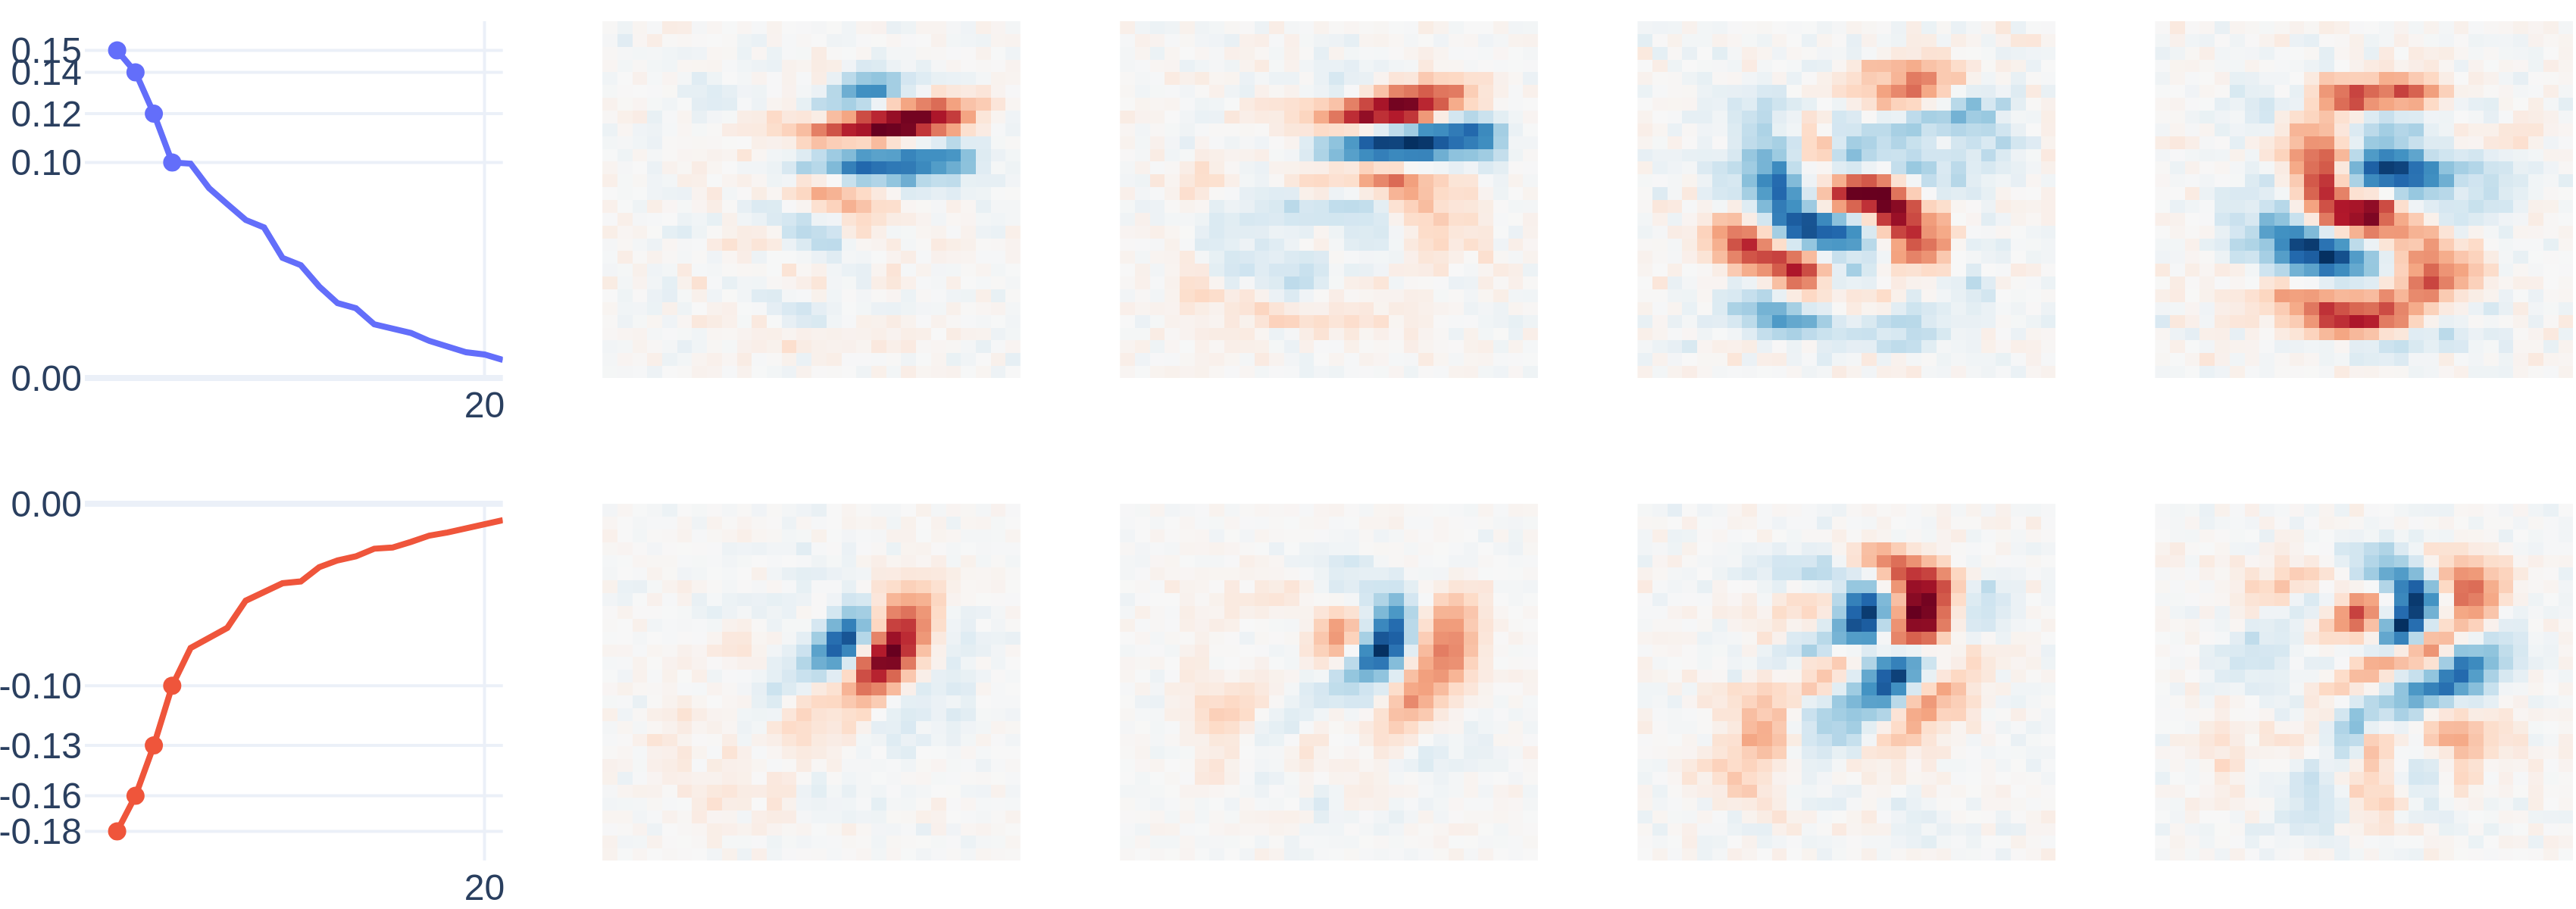
\includegraphics[width=0.75\linewidth]{figures/fig_03.png}
\end{center}
\caption{Reproduction of Figures~2B and~3 of \citet{pearce2025bilinear}. Top: the top
positive eigenvector for classes 1--5 of MNIST (upper row) and Fashion-MNIST (lower
row). Bottom: eigenvalue spectrum and top four positive (upper) and negative (lower)
eigenvectors for digit~5. Red and blue denote regions of opposite sign.}
\label{fig:c1}
\end{figure}

\subsection{C2: the computation is effectively low-rank and stable across runs}

We train five seeds at each of six hidden sizes and compare eigenvectors across
seeds. The top positive eigenvector reaches a mean cross-seed cosine similarity
between 0.73 and 0.88 depending on model size, declining with eigenvector rank, and
larger models remain similar deeper into the spectrum (rank-15 similarity 0.13 for
size 30 versus 0.48 for size 1000). Both the levels and the ordering match the
original Figure~5A. One protocol detail differs: we exclude the diagonal when
averaging over seed pairs, since comparing a run with itself contributes a constant
similarity of one; the original figure's slightly higher values are consistent with
this difference.

Truncating each classifier to its top-$k$ eigenvectors per class via
Equation~\ref{eq:eig} preserves accuracy with remarkably few components: at $k = 15$
the accuracy drop ranges from 0.01\% (size 30) to 1.4\% (size 1000), and by $k = 30$
all sizes are within noise of their full accuracy (94.8\% to 98.5\% across sizes).
This matches the original Figure~5B and Appendix~F. Figure~\ref{fig:c2} shows both
panels.

\begin{figure}[t]
\begin{center}
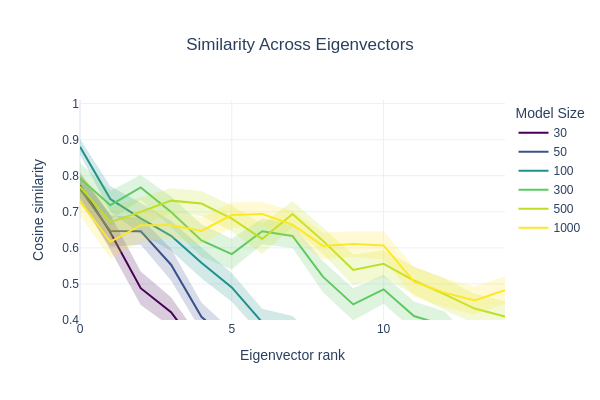
\includegraphics[width=0.48\linewidth]{figures/fig_05a.png}
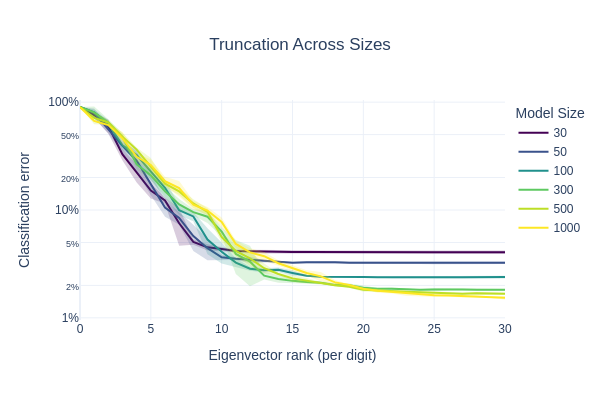
\includegraphics[width=0.48\linewidth]{figures/fig_05b.png}
\end{center}
\caption{Reproduction of Figure~5 of \citet{pearce2025bilinear}. Left: mean
cross-seed cosine similarity of eigenvectors by rank, for six model sizes (five seeds
each, diagonal pairs excluded, 90\% confidence bands). Right: classification error
after truncating each model to its top-$k$ eigenvectors per digit.}
\label{fig:c2}
\end{figure}

\subsection{C3: regularization controls the character of the features}

Sweeping the training-time Gaussian input noise from 0 to 0.8 reproduces the
qualitative transition of the original Figure~4: without noise the top eigenvector of
an unregularized model concentrates on scattered outlying pixels, a visible signature
of overfitting, and increasing noise produces progressively cleaner, more digit-like
features at essentially unchanged test accuracy (97.2\%--98.1\% across the sweep;
Figure~\ref{fig:c3}). The augmentation ablations of the original Appendix~B
reproduce as well: translation splits features into copies at multiple positions,
rotation broadens them, and blur smooths them, while none of the geometric
augmentations alone removes the edge-pixel overfitting that input noise removes. The
sparsity grid of the original Appendix~E confirms the quantitative half of the claim:
$(L_1/L_2)^2$ near-sparsity of the top-5 eigenvectors is governed almost entirely by
input noise, while the analogous statistic of the eigenvalue spectrum, the effective
rank, is reduced by weight decay.

\begin{figure}[t]
\begin{center}
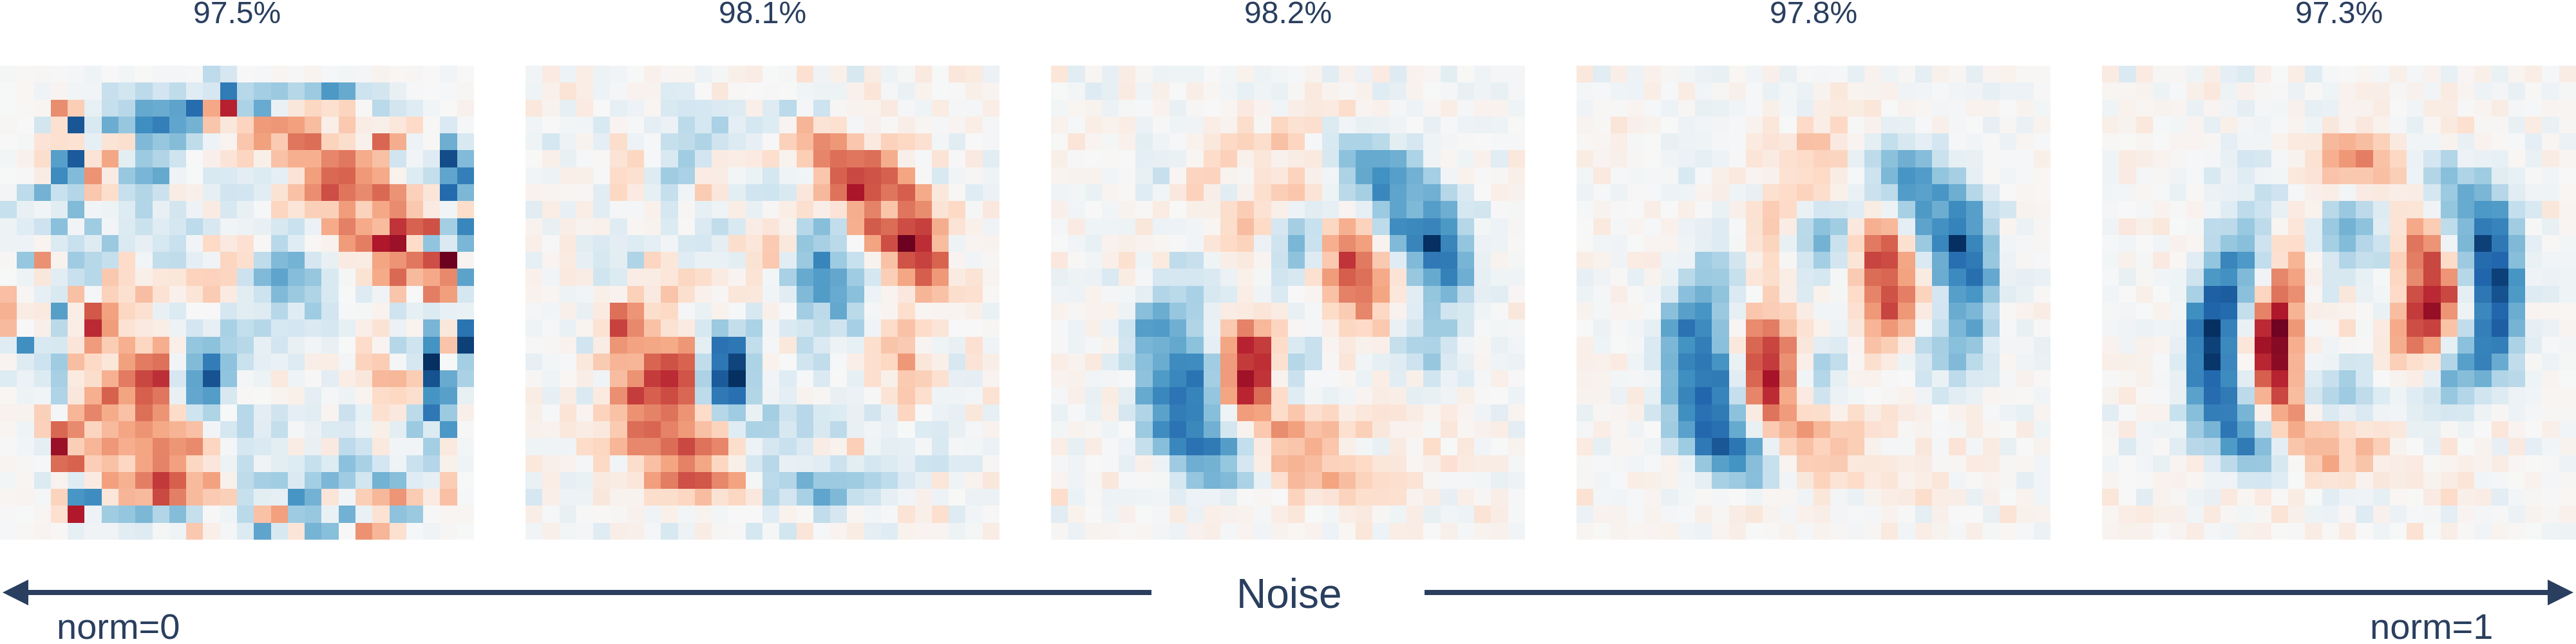
\includegraphics[width=0.95\linewidth]{figures/fig_04.png}
\end{center}
\caption{Reproduction of Figure~4 of \citet{pearce2025bilinear}: the top eigenvector
of digit~0 for models trained with increasing Gaussian input noise (left to right),
annotated with test accuracy. Overfitting artifacts on rarely active pixels disappear
as noise increases.}
\label{fig:c3}
\end{figure}

\subsection{C4: weight-derived masks causally steer the model}

We reproduce the pseudoinverse-mask construction of the original Figure~7: for each
class, the rows of the pseudoinverse of its top-10 eigenvectors act as keys that
activate specific eigenvectors, and adding a scaled key to every test image steers
the model toward the corresponding class. Evaluated on the full test set, a mask of
standard deviation 0.3 built for a noise-regularized model (input noise 0.15) drops
accuracy from 97.9\% to 58.7\% while a permuted version of the same mask leaves it at
95.6\%, and raises targeted misclassification to 28.7\% against 0.6\% for the random
baseline (Figure~\ref{fig:c4}). For an unregularized model the second variant of the
experiment restricts masks to border pixels active in under 1\% of samples, purely
exploiting the overfitting structure visible in C3, and still drops accuracy from
97.6\% to 23.5\% (random baseline 40.5\%).

The original Appendix~M studies how mask effectiveness varies with regularization,
and our quantitative version confirms its message: as training noise increases from 0
to 0.3, the same attack at mask strength 0.3 recovers from 31.8\% to 74.4\% accuracy,
with random-mask baselines between 85.9\% and 97.2\% throughout, so weight-derived
masks remain far more effective than chance even against the most regularized model.

\begin{figure}[t]
\begin{center}
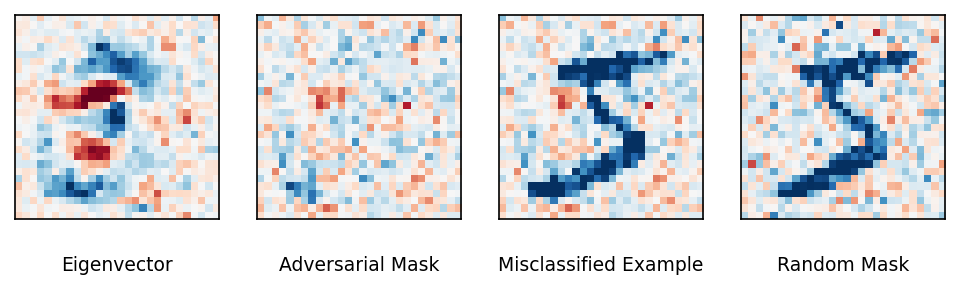
\includegraphics[width=0.7\linewidth]{figures/fig_07a1.png}\\[2pt]
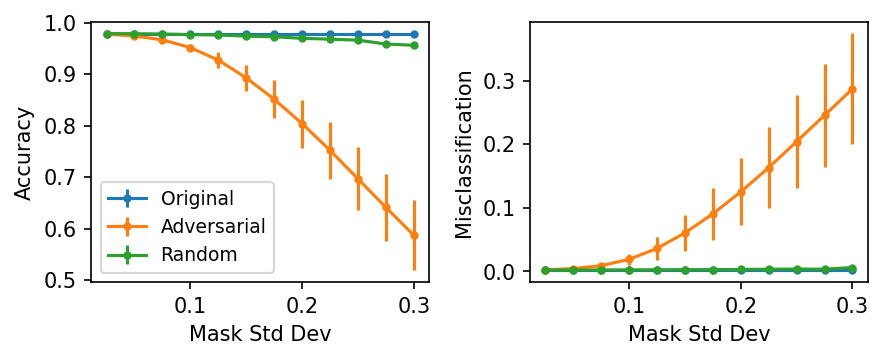
\includegraphics[width=0.7\linewidth]{figures/fig_07b1.png}
\end{center}
\caption{Reproduction of Figure~7 of \citet{pearce2025bilinear} (noise-regularized
model). Top: an eigenvector for digit~3, its pseudoinverse-based adversarial mask, a
misclassified example, and a permuted random mask. Bottom: test-set accuracy and
targeted misclassification as functions of mask strength, for adversarial and random
masks.}
\label{fig:c4}
\end{figure}

\subsection{C5: the sentiment-negation circuit is recoverable from the weights}

Using the public 6-layer TinyStories model and its layer-4 SAEs, we contract the
bilinear tensor with the encoder direction of the ``not-good'' output feature
(index 1882) and transform the interaction matrix into the input SAE feature basis.
The reproduced interaction submatrix (Figure~\ref{fig:c5}, left) shows the AND-gate
structure of the original Figure~8A: negative-sentiment input features interact
strongly and positively with negation features while both groups have negligible
self-interactions, and the one positive-sentiment feature interacts with the opposite
sign. Projecting the input features onto the top positive and negative eigenvectors
of the interaction matrix (Figure~\ref{fig:c5}, right) reproduces the circuit
geometry of Figure~8B, including the positions of the ``bad''$-$``good'' unembedding
difference and the residual-stream activation of an isolated ``not'' token. The two
outlier eigenvalues of the interaction matrix reproduce exactly at the paper's
reported precision, $+0.62$ and $-0.66$, as expected for quantities computed from
the weights alone. The rank-2 approximation of the feature's activation via
Equation~\ref{eq:eig} concentrates along the diagonal at large activations, as in
the original Figure~8C, with an active-only correlation of 0.54 against the paper's
0.66; unlike the eigenvalues, this statistic depends on the evaluation corpus, and
ours necessarily differs (Section~\ref{sec:deviations}). The interaction histogram
of the original Appendix~N reproduces as well, and the top-activating text examples
for all thirteen circuit features (original Appendix~O) match the published feature
labels.

\begin{figure}[t]
\begin{center}
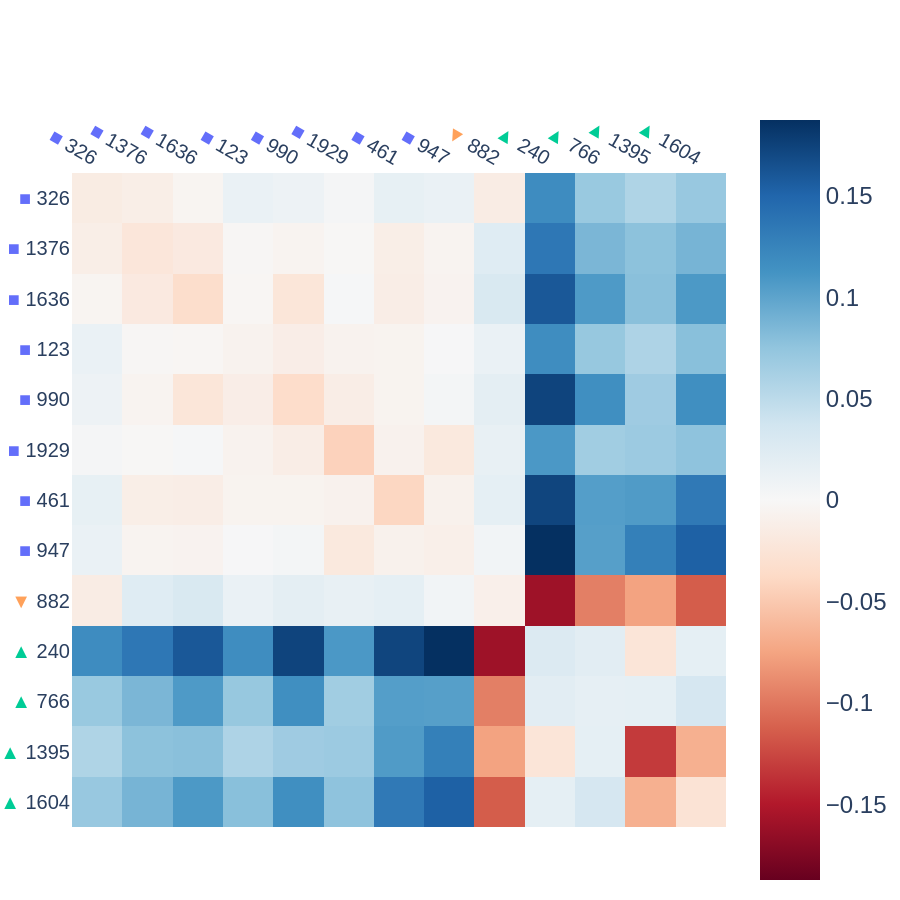
\includegraphics[width=0.42\linewidth]{figures/fig_08a.png}
\hspace{8pt}
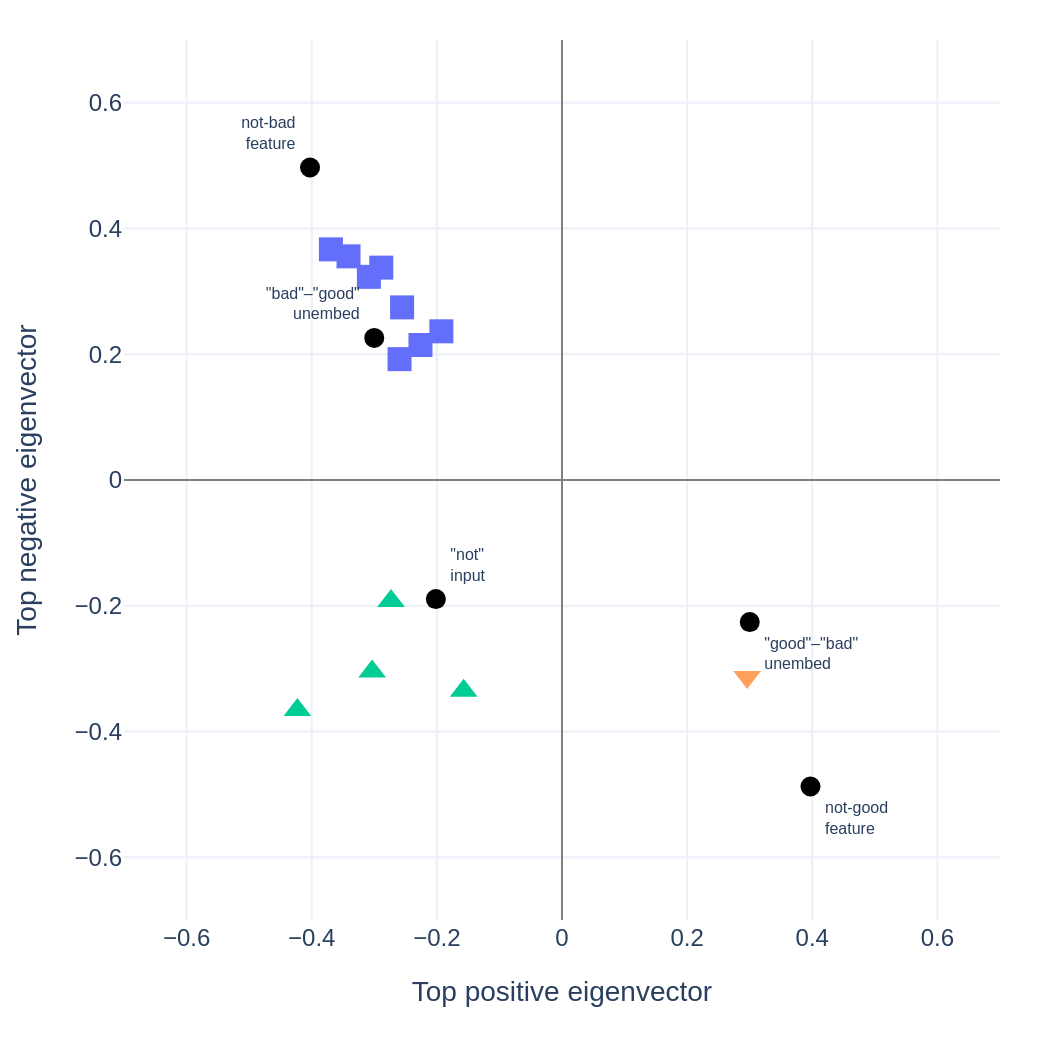
\includegraphics[width=0.42\linewidth]{figures/fig_08b.png}
\end{center}
\caption{Reproduction of Figure~8 of \citet{pearce2025bilinear}. Left: interaction
submatrix of the top interactions computing the ``not-good'' feature; squares mark
negative-sentiment input features, triangles negation features. Right: projection of
input features and anchor directions onto the top positive and negative
eigenvectors.}
\label{fig:c5}
\end{figure}

\subsection{C6: language-model features are low-rank}

Figure~\ref{fig:c6} reproduces Figure~9 of the original across the three
transformers. For fw-medium, the mean correlation between an SAE feature's activation
and its truncated eigendecomposition rises from 0.51 with one eigenvector to 0.83
with 64; 74\% of features exceed a correlation of 0.75 with only the top two
eigenvectors, matching the original's statement that most features do. Scatter plots
of nine randomly sampled features show the activation concentrating on the diagonal
(correlations 0.75--0.96 for eight of nine), with one densely activating feature
poorly approximated, mirroring the heterogeneity visible in the original Figure~9C.
One ordering detail differs: in our run fw-small attains slightly higher correlations
than fw-medium, whereas the original reports the reverse; both lie in the reported
range.

The training-time effect of the original Appendix~H reproduces closely with the five
released SAE snapshots of doubling training duration: our mean correlations are
0.19, 0.30, 0.47, 0.57 and 0.62 against the paper's Table-5 values of
0.17, 0.28, 0.42, 0.52 and 0.59, and the correlation histogram shifts from a bimodal
shape with most mass near zero to a single mode near 0.85, as in the original
Figure~24. Finally, the SAE quality curve of the original Appendix~G (loss added when
splicing each SAE's reconstruction into the forward pass) reproduces in its ordering,
with resid-mid costing more than mlp-out at every layer, but its absolute values are
distorted by an evaluation-data mismatch discussed in Section~\ref{sec:deviations};
we therefore additionally report per-layer reconstruction error, which rises
monotonically with depth for both hook points, consistent with the original figure.

\begin{figure}[t]
\begin{center}
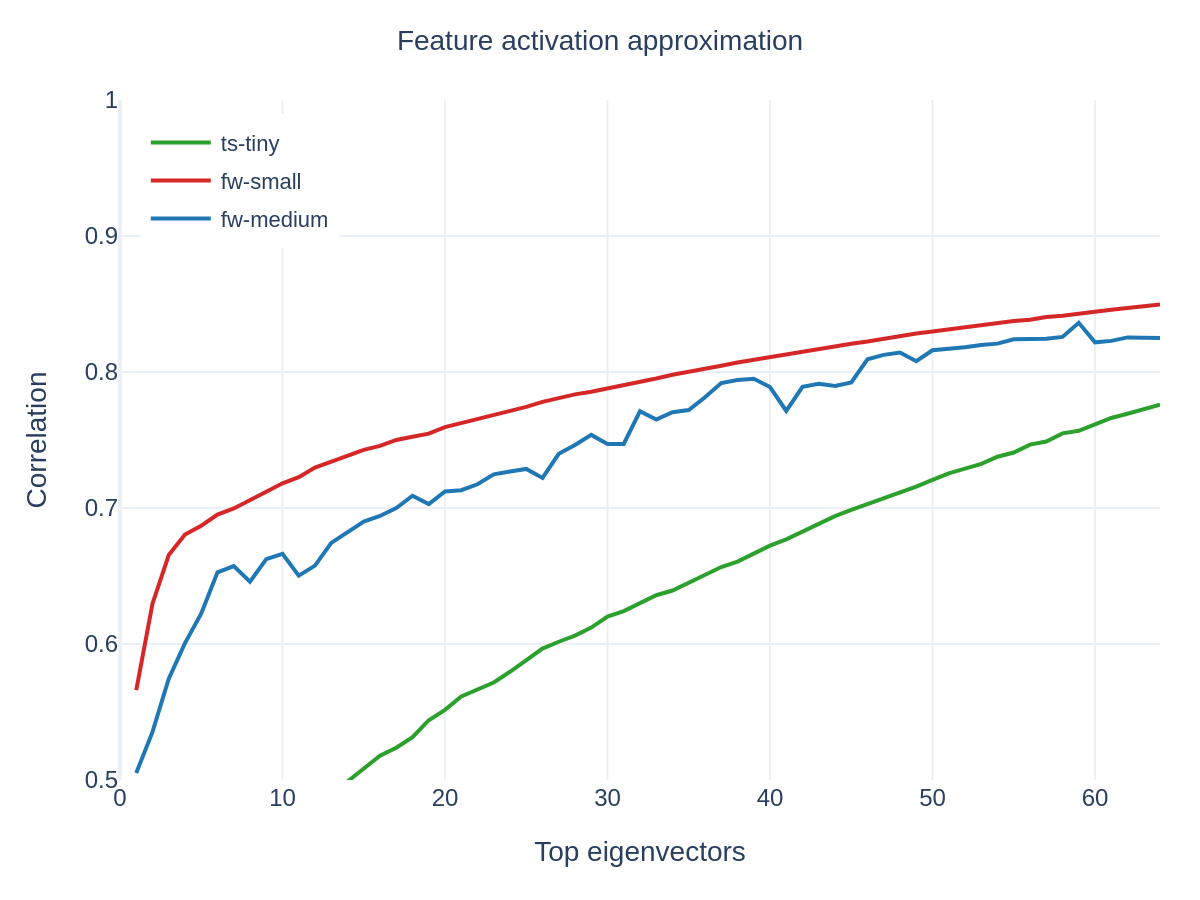
\includegraphics[width=0.48\linewidth]{figures/fig_09a.png}
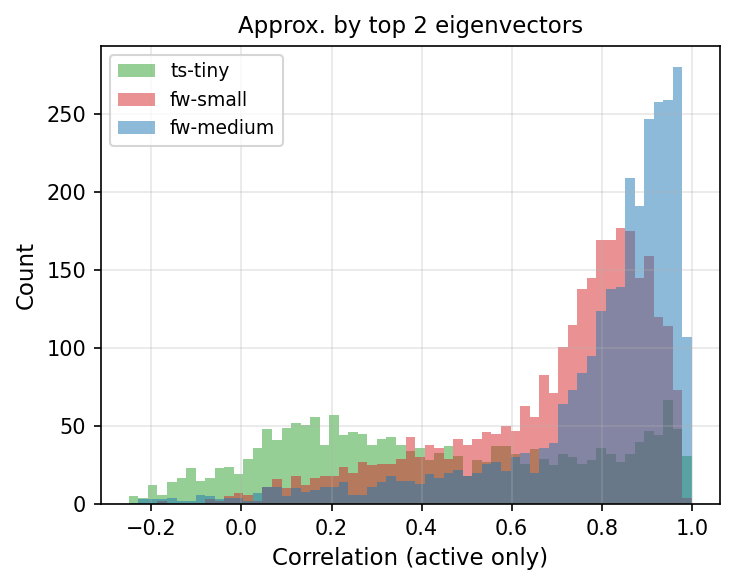
\includegraphics[width=0.44\linewidth]{figures/fig_09b.png}\\[4pt]
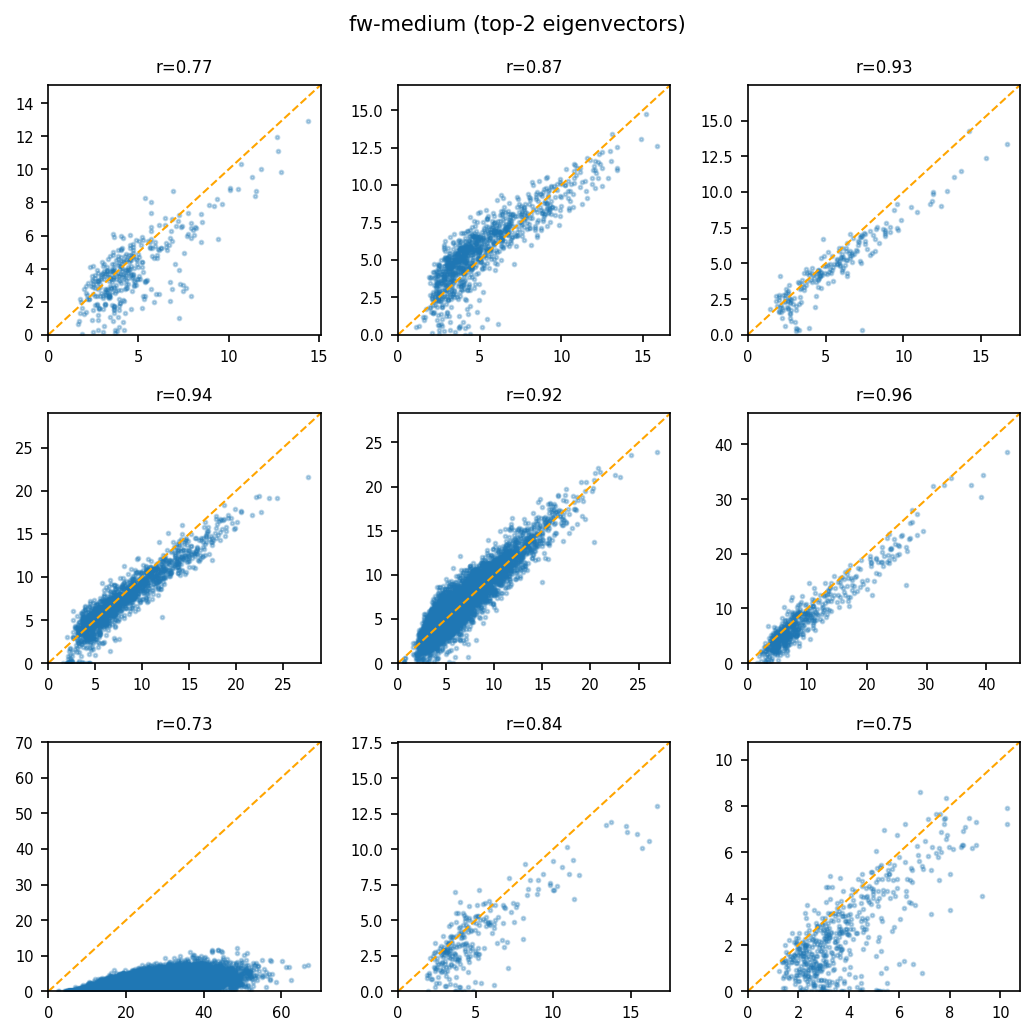
\includegraphics[width=0.5\linewidth]{figures/fig_09c.png}
\end{center}
\caption{Reproduction of Figure~9 of \citet{pearce2025bilinear}. Top left: mean
correlation between SAE feature activations and truncated eigendecomposition
approximations, as a function of the number of eigenvectors. Top right: distribution
of per-feature correlations using the top two eigenvectors. Bottom: activation versus
rank-2 approximation for nine randomly sampled fw-medium features.}
\label{fig:c6}
\end{figure}

\subsection{C7: bilinear layers as a drop-in replacement}

We train three 6-layer TinyStories transformers from scratch, identical except for
the MLP activation, and derive both rows of the original Table~6 from one set of
runs: the constant-epochs comparison from the final validation loss, and the
constant-time comparison from timestamped periodic validation evaluated at the
wall-clock time when the fastest variant finished. Table~\ref{tab:c7} reports the
result. The core of the claim reproduces: after five epochs the bilinear model
trails SwiGLU by only 0.006 nats (1.237 against 1.231), the same order as the
paper's 0.016 gap, and is indistinguishable from ReGLU; at constant time the
bilinear model sits between the two gated variants, 0.005 nats behind SwiGLU. The
full constant-time equalization of the original Table~6 did not manifest, for a
mechanical reason: in our implementation the three variants run at nearly identical
wall-clock speed (the gate is a negligible element-wise operation), so constant
time buys the slower variants almost no extra steps. The original's own footnote
anticipates this, noting that the constant-time result depends on implementation
efficiency.
Because our runs use the public TinyStories corpus rather than the authors'
unavailable cleaned version, absolute losses are not comparable to the original;
the claim concerns the differences between activation functions, which we measure
under identical conditions.

For the fine-tuning half of the claim we anneal TinyLlama-1.1B's gate away over the
first 30\% of a 100{,}000-step run on roughly 400M FineWeb tokens
(Figure~\ref{fig:c7}). The loss trajectory reproduces the shape of the original
Figure~25: the fine-tuned arm tracks the continued-training baseline during early
annealing, rises to a gap of about 0.2 nats as $\beta$ approaches zero, and recovers
steadily under continued training, ending 0.14 nats above the baseline (2.49 against
2.35) after 400M tokens, against the paper's residual gap of 0.05. Two factors
plausibly account for the larger residual: our stability-driven lower learning rate
slows recovery, and our compute budget matches the paper's token count, which its
authors already describe as insufficient for full convergence. The qualitative
conclusion, that a pretrained gated transformer can be converted to a bilinear one at
a modest and shrinking penalty, stands.

\begin{table}[t]
\caption{Validation loss of TinyStories transformers with different MLP activations
(our runs, public TinyStories corpus; paper values in parentheses for reference,
measured on the authors' unavailable cleaned corpus). The constant-epochs row
reports the final loss on the full validation set; the constant-time row evaluates
each variant on a fixed 1024-sequence validation subset at the wall-clock time when
the fastest variant finished.}
\label{tab:c7}
\begin{center}
\begin{tabular}{lccc}
\toprule
 & Bilinear & ReGLU & SwiGLU \\
\midrule
constant epochs & 1.237 (1.337) & 1.242 (1.332) & 1.231 (1.321) \\
constant time   & 1.228 (1.337) & 1.231 (1.337) & 1.223 (1.336) \\
\bottomrule
\end{tabular}
\end{center}
\end{table}

\begin{figure}[t]
\begin{center}
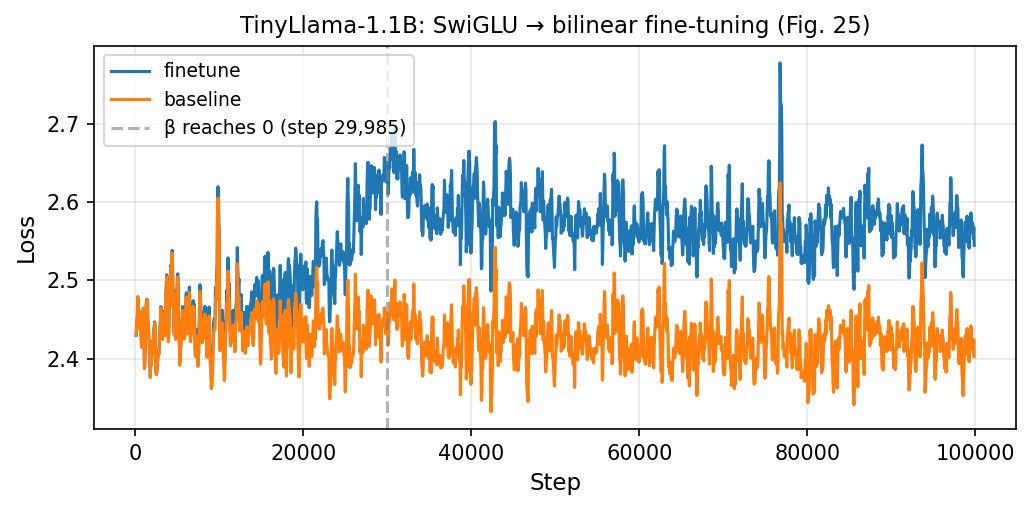
\includegraphics[width=0.75\linewidth]{figures/fig_25.png}
\end{center}
\caption{Reproduction of Figure~25 of \citet{pearce2025bilinear}: fine-tuning
TinyLlama-1.1B while annealing the SwiGLU gate to the identity ($\beta \to 0$ over
the first 30\% of steps), against a continued-training baseline. The conversion
penalty peaks near the end of annealing and shrinks with continued training.}
\label{fig:c7}
\end{figure}

\subsection{Results beyond the original paper}
\label{sec:extension}

% EXTENSION SECTION — to be written later (bilinear VAE study).

\section{Discussion}
\label{sec:discussion}

\subsection{What the reproduction supports}

The central methodological claim of \citet{pearce2025bilinear} holds up well under
independent reproduction: for bilinear MLPs, the weights alone support analyses that
normally require data, and the structures they reveal are real in the strongest
available sense, since masks derived purely from eigenvectors steer the model (C4)
and eigenvector approximations track SAE feature activations on held-out text (C6).
We found the vision results robust to full retraining from scratch, including their
quantitative details, and the language results reproducible from the released
checkpoints and dictionaries.

\subsection{Deviations and their causes}
\label{sec:deviations}

We record four deviations, each traced to its cause.

\paragraph{The cleaned TinyStories dataset is unavailable.} The published
TinyStories checkpoint reaches a per-token loss of about 2.9 on the public
TinyStories validation set, against the 1.34 the paper reports on the authors'
cleaned corpus. We ruled out our evaluation pipeline as the cause by testing
tokenization and punctuation normalization, story packing and padding conventions,
attention masking, and rotary embedding variants; none moves the number
appreciably, and the same evaluation applied to our own from-scratch models
produces losses in the expected range (Table~\ref{tab:c7}). The gap therefore
reflects a genuinely different training distribution that can no longer be
obtained, since the research repository that produced it is no longer public. Most
results are unaffected, but one is: the loss-added metric of the original
Appendix~G evaluates the model slightly off its training distribution, where an SAE
reconstruction can act as a denoiser, compressing and occasionally inverting the
metric's absolute values. The ordering between hook points survives; the absolute
curve does not.

\paragraph{Fine-tuning diverges at the reported learning rate.} The original
Appendix~J describes fine-tuning TinyLlama with the FineWeb configuration of the
paper's Table~3, whose learning rate of $6 \times 10^{-4}$ is a from-scratch
pretraining value. At our batch size of 4096 tokens per step, both the fine-tuning
arm and the continued-training baseline diverge immediately after warmup at that
rate, from loss 2.7 to above 7. At $3 \times 10^{-5}$ both arms train stably. We
report results at the stable rate and flag the discrepancy.

\paragraph{Protocol details.} Two smaller items: our cross-seed similarity curves
(C2) exclude self-pairs from the average, which lowers the curves slightly relative
to including them; and in C6 the ordering of fw-small and fw-medium is swapped
relative to the original, within the reported range.

\paragraph{Software drift.} The vendored library predates breaking changes in its
dependencies: current \texttt{transformers} drops non-registered buffers when
loading the released checkpoints, requiring the attention mask and rotary caches to
be rebuilt after loading, and current PyTorch rejects the training-path attention
call, which passes an explicit mask together with \texttt{is\_causal}. Our scripts
carry small, documented shims for both. Neither affects results; both would stop a
naive rerun.

\subsection{What was easy and what was difficult}

The vision experiments were straightforward: the library's decomposition code is
clean, models train in minutes, and the paper describes the setups precisely enough
to re-implement every figure. The language experiments were harder for reasons that
have little to do with the method. The missing research repository meant all
experiment code had to be reconstructed from prose; the missing cleaned dataset put
absolute loss comparisons permanently out of reach; and locating the correct public
artifacts required some detective work, for instance the paper's ``ts-tiny'' model
being published under the name \texttt{ts-medium}. A general lesson we would pass to
authors of interpretability papers: releasing trained checkpoints and dictionaries,
as these authors did, enables most of a reproduction, but the training corpus and
the experiment scripts are what make loss-based claims checkable.

\subsubsection*{Broader Impact Statement}

This work evaluates and extends an interpretability method; it introduces no new
model capabilities. The adversarial masks of C4 are constructed from full knowledge
of a model's weights and target small MNIST classifiers, so they do not constitute a
practical attack surface beyond what gradient-based attacks already provide in the
white-box setting. We expect the net impact of better weight-based transparency
tools to be positive.

\bibliography{main}
\bibliographystyle{tmlr}

\appendix

\section{Model architectures and hyperparameters}
\label{app:hyper}

\begin{table}[h]
\caption{Vision model training configuration (all C1--C4 experiments unless the
experiment sweeps the parameter).}
\begin{center}
\begin{tabular}{ll}
\toprule
input / hidden / output & $784$ / $512$ / $10$ \\
biases & none \\
optimizer & AdamW, lr $10^{-3}$, weight decay $1.0$ \\
schedule & cosine annealing \\
batch size & 2048 \\
epochs & 50--100 \\
input noise & Gaussian, std $0.5$ \\
\bottomrule
\end{tabular}
\end{center}
\end{table}

\begin{table}[h]
\caption{TinyStories transformer configuration (public checkpoint and our C7 runs).}
\begin{center}
\begin{tabular}{ll}
\toprule
layers / $d_{\text{model}}$ / $d_{\text{hidden}}$ / heads & 6 / 512 / 2048 / 8 \\
context / vocabulary & 256 / 4096 (lowercase BPE) \\
optimizer & AdamW, lr $10^{-3}$, weight decay $0.1$, $\beta = (0.9, 0.95)$ \\
schedule & linear warmup (50 steps), linear decay \\
batch size & 512 sequences \\
epochs & 5 \\
\bottomrule
\end{tabular}
\end{center}
\end{table}

\begin{table}[h]
\caption{TinyLlama fine-tuning configuration (C7).}
\begin{center}
\begin{tabular}{ll}
\toprule
model & TinyLlama-1.1B (bfloat16) \\
data & FineWeb sample-10BT, packed to 512 tokens \\
steps / tokens & 100{,}000 / $\approx$ 409M \\
batch & 4096 tokens per optimizer step \\
optimizer & AdamW, lr $3 \times 10^{-5}$, weight decay 0.1, $\beta = (0.9, 0.95)$ \\
$\beta$-annealing & linear $1 \to 0$ over first 30\% of steps \\
\bottomrule
\end{tabular}
\end{center}
\end{table}

\section{Additional reproduced material}
\label{app:extra}

Beyond the figures shown in the main text, the repository reproduces: per-digit
eigenspectra for all MNIST classes (original Appendix~A); the augmentation grids for
blur, rotation and translation (original Appendix~B, Figure~14); per-example
explanations of a correctly and an incorrectly classified digit (original
Appendix~C); the HOSVD decomposition of the full bilinear tensor (original
Appendix~D, Figures~17--18); the sparsity grids over weight decay and input noise
(original Appendix~E, Figure~19); the reverse-engineering of the
similarity-classifier challenge including the learned bias (original Figure~6);
adversarial masks under three regularization levels with quantitative baselines
(original Appendix~M); the interaction histogram and eigenvalue spectrum of the
negation feature (original Appendix~N, Figure~27); and the top-activating text
examples of all circuit features (original Appendix~O, Tables~7--9). Each experiment
directory contains the corresponding figures and, where applicable, a JSON file with
the quantitative results.

\end{document}
